\chapter{Acción estacionaria y ecuación de Euler--Lagrange}

\lectureoverview{El nombre familiar «\emph{principio de mínima acción}» oculta la idea esencial: la trayectoria física hace estacionaria la acción, pero no tiene por qué minimizarla. Partiremos del equilibrio ordinario y extenderemos esa idea de puntos a funciones consideradas en su totalidad, deduciremos la ecuación de Euler--Lagrange discretizando una trayectoria y recuperaremos las ecuaciones de Newton. Después, las coordenadas giratorias y polares mostrarán por qué la formulación lagrangiana es más que un cambio de notación.}

\section{Estacionaria, no necesariamente mínima}

La palabra «\emph{mínima}» es la parte poco fiable del nombre tradicional. Una trayectoria clásica no siempre hace mínima la acción. En su lugar, puede corresponder a un máximo o a un punto de silla en el espacio de trayectorias posibles. El principio correcto establece que la acción es \emph{estacionaria}: su variación de primer orden se anula.

Empecemos con la cuestión más sencilla del equilibrio. Una partícula que permanece en reposo no tiene aceleración, así que la fuerza neta debe anularse. Para una fuerza derivada de un potencial unidimensional,\begin{equation}
  F(x)=-\frac{dV}{dx},
  \label{eq:force-from-v}
\end{equation}la condición de equilibrio es\begin{equation}
  \frac{dV}{dx}=0.
  \label{eq:stationary-v-one}
\end{equation}

\begin{figure}[htbp]
  \centering
  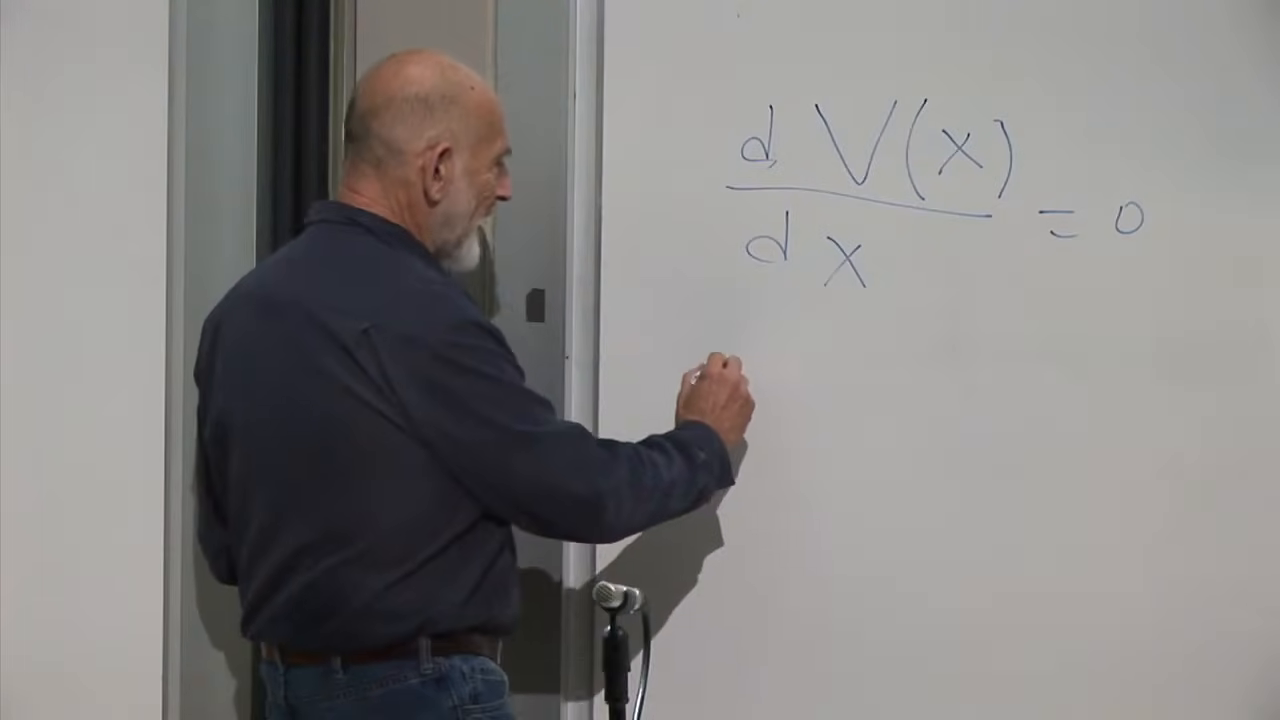
\includegraphics[width=0.74\textwidth]{lecture_03_figure_02.png}
  \caption{Condición de equilibrio unidimensional: la fuerza se anula donde el potencial es estacionario.}
  \lectureframe{00:02:51}
\end{figure}

Desplacemos ahora la partícula una pequeña cantidad \(\delta x\). A primer orden,\begin{equation}
  \delta V
  =V(x+\delta x)-V(x)
  =\frac{dV}{dx}\,\delta x+O(\delta x^2).
  \label{eq:first-variation-one}
\end{equation}En el equilibrio, el término lineal se anula para cualquiera de los dos signos de \(\delta x\):\begin{equation}
  \delta V=0
  \qquad\hbox{to first order.}
  \label{eq:delta-v-zero-one}
\end{equation}Esto no significa que \(V\) permanezca exactamente inalterado tras un desplazamiento finito. Significa que el cambio dominante es cuadrático o de orden superior. Tanto un mínimo como un máximo satisfacen esta condición.

\begin{figure}[htbp]
  \centering
  \begin{tikzpicture}[scale=0.95,>=Latex]
    \draw[->] (-0.2,0) -- (3.35,0) node[right] {$x$};
    \draw[->] (0,-0.2) -- (0,2.25) node[above] {$V$};
    \draw[blue!65!black,thick,smooth]
      plot coordinates {(0.2,1.85) (0.75,0.85) (1.55,0.35)
                        (2.35,0.85) (3.0,1.85)};
    \fill[red!65!black] (1.55,0.35) circle (2pt);
    \node at (1.55,-0.34) {minimum};
    \begin{scope}[xshift=4.25cm]
      \draw[->] (-0.2,0) -- (3.35,0) node[right] {$x$};
      \draw[->] (0,-0.2) -- (0,2.25) node[above] {$V$};
      \draw[blue!65!black,thick,smooth]
        plot coordinates {(0.2,0.35) (0.75,1.25) (1.55,1.85)
                          (2.35,1.25) (3.0,0.35)};
      \fill[red!65!black] (1.55,1.85) circle (2pt);
      \node at (1.55,-0.34) {maximum};
    \end{scope}
  \end{tikzpicture}
  \caption{La estacionariedad fija la primera derivada, pero no determina si el punto es un mínimo o un máximo.}
  \label{fig:min-max-stationary}
\end{figure}

Para muchas coordenadas \(q_i\), la primera variación es\begin{equation}
  \delta V
  =\sum_i\frac{\partial V}{\partial q_i}\,\delta q_i.
  \label{eq:first-variation-many}
\end{equation}Si debe anularse para todo desplazamiento infinitesimal independiente \(\delta q_i\), entonces se anula cada coeficiente:\begin{equation}
  \frac{\partial V}{\partial q_i}=0
  \qquad\hbox{for every }i.
  \label{eq:stationary-v-many}
\end{equation}

Es mejor imaginar un potencial bidimensional como un terreno ondulado que como una montaña rusa. Un punto estacionario puede ser el fondo de un valle, la cima de una colina o un punto de silla. En un punto de silla, el movimiento inicialmente asciende en una dirección y desciende en otra. Por tanto, el comportamiento restaurador puede ser estable en una dirección e inestable en otra, aunque todas las primeras derivadas se anulen en el punto mismo.

\begin{figure}[htbp]
  \centering
  \includegraphics[width=0.76\textwidth]{lecture_03_figure_06.png}
  \caption{Un punto de silla es estacionario en todas las direcciones a primer orden, aunque los desplazamientos cercanos asciendan a lo largo de un eje y desciendan a lo largo de otro.}
  \lectureframe{00:08:20}
\end{figure}

En un espacio con muchas coordenadas, los puntos de silla son más habituales que los máximos o mínimos puros. Por eso, «\emph{estacionario}» es el término que conviene usar. La condición\begin{equation}
  \delta V=0
  \label{eq:equilibrium-variation}
\end{equation}resume el equilibrio sin prejuzgar el comportamiento de segundo orden.

\section{De los puntos a las funciones}

La mecánica estudia movimientos completos, no puntos de equilibrio aislados. Una trayectoria es una función como \(x(t)\), o una colección de funciones \((x(t),y(t),z(t))\). El problema matemático de hacer estacionaria una cantidad variando una función entera se llama \emph{cálculo de variaciones}. Antes de aplicarlo al movimiento, consideremos tres ejemplos más sencillos.

\subsection{Curvas más cortas y geodésicas}

Fijemos dos puntos del plano y representemos mediante \(y(x)\) una curva que los une. Para un segmento corto,\begin{equation}
  ds=\sqrt{dx^2+dy^2}
  =dx\sqrt{1+\left(\frac{dy}{dx}\right)^2},
  \label{eq:line-element}
\end{equation}donde la última expresión supone que \(dx>0\). La longitud total es el funcional\begin{equation}
  S[y]=\int_{x_0}^{x_1}
  \sqrt{1+y'(x)^2}\,dx.
  \label{eq:arc-length-functional}
\end{equation}Los corchetes resaltan que \(S\) toma como entrada una función entera. La recta queda seleccionada por\begin{equation}
  \delta S=0
  \label{eq:stationary-length}
\end{equation}entre pequeñas variaciones de la curva que mantienen fijos ambos extremos.

\begin{figure}[htbp]
  \centering
  \includegraphics[width=0.78\textwidth]{lecture_03_figure_07.png}
  \caption{Curva de prueba entre dos extremos fijos. Su longitud es la suma de las hipotenusas infinitesimales \(ds\).}
  \lectureframe{00:13:36}
\end{figure}

La misma pregunta puede plantearse sobre una superficie curva. Tensar una cuerda entre dos estacas da una imagen física de la ruta más corta sujeta a esas restricciones. Una curva de longitud estacionaria de este tipo es una \emph{geodésica}. En un plano llano es una recta; sobre una esfera o una superficie ondulada, por lo general no lo es.

\subsection{Principio de Fermat}

Un rayo de luz en un medio donde la rapidez depende de la posición \(c(x,y)\) no tiene por qué seguir la ruta espacial más corta. El tiempo que tarda en recorrer un segmento pequeño es la distancia dividida por la rapidez local, de modo que\begin{equation}
  T[y]
  =\int_{x_0}^{x_1}
  \frac{\sqrt{1+y'(x)^2}}{c(x,y)}\,dx.
  \label{eq:fermat-functional}
\end{equation}El principio de Fermat exige que\begin{equation}
  \delta T=0.
  \label{eq:fermat-stationary}
\end{equation}Cuando \(c\) es constante, esto se reduce al problema de la distancia mínima. Sin embargo, en un medio con índice de refracción variable, la trayectoria más rápida equilibra la distancia con la rapidez de propagación local.

\begin{figure}[htbp]
  \centering
  \includegraphics[width=0.80\textwidth]{lecture_03_figure_08.png}
  \caption{Funcional del tiempo mínimo para un rayo en un medio cuya rapidez local de la luz depende de la posición.}
  \lectureframe{00:22:50}
\end{figure}

Un chiste de actualidad alude a la afirmación, por entonces reciente, de que los neutrinos se movían a una velocidad inusualmente alta en Italia. El argumento físico vuelve enseguida al ejemplo fiable: la luz ordinaria cambia de rapidez en los materiales según el índice de refracción.

\subsection{Una cadena colgante}

Una cadena sujeta en dos puntos adopta la forma de una catenaria. Cada pequeño tramo contribuye a la energía potencial gravitatoria, por lo que el potencial total es, a su vez, una integral sobre la cadena. Una vez más, los extremos están fijos, la forma desconocida es una función y una integral debe ser estacionaria.

\begin{figure}[htbp]
  \centering
  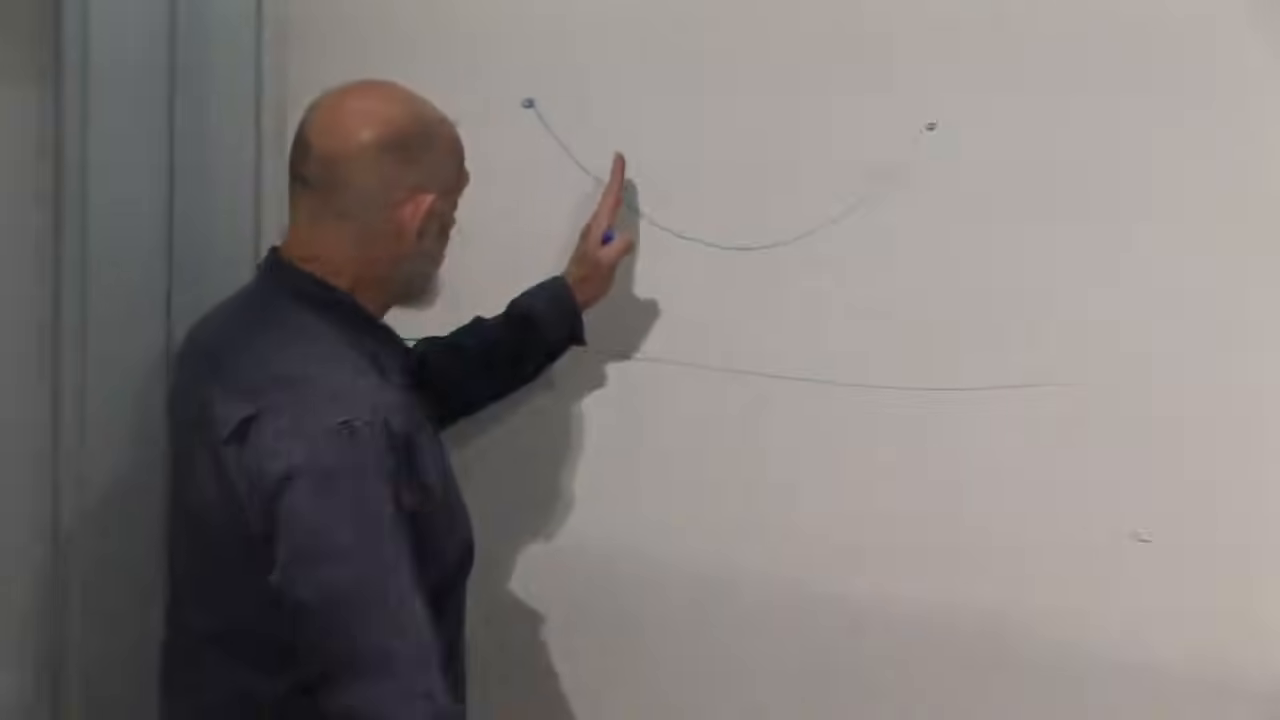
\includegraphics[width=0.76\textwidth]{lecture_03_figure_03.png}
  \caption{Cadena colgante entre soportes fijos. Su forma estacionaria queda determinada por la energía potencial gravitatoria total.}
  \lectureframe{00:30:41}
\end{figure}

Estos ejemplos tienen la misma estructura: dos extremos fijos, una función entre ellos y una integral cuya primera variación se anula. Reducir una condición global de este tipo a una ecuación diferencial es lo que significa resolver el problema variacional.

\section{La mecánica como problema de contorno}

A menudo se representa la trayectoria con el tiempo en el eje horizontal porque \(t\) es la variable independiente. Sin embargo, en física existe una marcada convención de dibujar el tiempo hacia arriba. Un comentario recuerda experimentos en los que se pidió a las personas ordenar imágenes desde la juventud hasta la vejez siguiendo las direcciones asociadas a sus sistemas de escritura: quienes leen de izquierda a derecha tendían a ordenarlas así; quienes leen de derecha a izquierda, en el sentido opuesto; y quienes están acostumbrados a la escritura vertical, verticalmente. El chiste concluye que los físicos son quienes insisten en que el tiempo fluye hacia arriba. Aquí usaremos el eje horizontal convencional \(t\) porque permite leer \(x(t)\) de forma natural como una gráfica.

En la formulación de valor inicial, los datos en \(t_0\) son\begin{equation}
  x(t_0)=x_0,
  \qquad
  \dot x(t_0)=v_0.
  \label{eq:initial-value-data}
\end{equation}La ecuación de Newton determina entonces la órbita posterior. La formulación variacional plantea un problema distinto: se especifican dos sucesos extremos,\begin{equation}
  x(t_0)=x_0,
  \qquad
  x(t_1)=x_1,
  \label{eq:boundary-value-data}
\end{equation}y se determina la trayectoria física entre ellos. La velocidad inicial ya no se proporciona; pasa a formar parte de la solución.

\begin{figure}[htbp]
  \centering
  \includegraphics[width=0.76\textwidth]{lecture_03_figure_09.png}
  \caption{Una trayectoria mecánica \(x(t)\). Se pueden especificar la posición y la pendiente en un extremo, o las posiciones en dos instantes extremos.}
  \lectureframe{00:27:41}
\end{figure}

La cantidad que debe hacerse estacionaria es la \emph{acción},\begin{equation}
  A[x]=\int_{t_0}^{t_1}L(x,\dot x,t)\,dt.
  \label{eq:action-one}
\end{equation}El integrando \(L\) es el \emph{lagrangiano}. Puede depender de la posición, la velocidad y el tiempo de forma explícita. El principio de acción establece que\begin{equation}
  \delta A=0
  \label{eq:stationary-action}
\end{equation}para todas las pequeñas variaciones de la trayectoria que cumplen\begin{equation}
  \delta x(t_0)=\delta x(t_1)=0.
  \label{eq:fixed-endpoint-variations}
\end{equation}La condición en los extremos es esencial: comparamos trayectorias vecinas que conectan los mismos dos sucesos.

\section{Una deducción discreta de la ecuación de Euler--Lagrange}

La acción es un funcional de infinitos valores de la trayectoria. Para concretar su variación, dividamos el intervalo de tiempo en pasos de longitud \(\epsilon\),\begin{equation}
  t_n=t_0+n\epsilon,
  \qquad
  x_n=x(t_n),
  \label{eq:discrete-times}
\end{equation}y aproximemos la velocidad en el intervalo \(n\) mediante\begin{equation}
  v_n=\frac{x_{n+1}-x_n}{\epsilon}.
  \label{eq:discrete-velocity}
\end{equation}La integral se convierte en la suma ordinaria\begin{equation}
  A_\epsilon
  =\sum_{n=0}^{N-1}
  \epsilon L\left(x_n,\frac{x_{n+1}-x_n}{\epsilon}\right).
  \label{eq:discrete-action}
\end{equation}Usamos \(n\) como etiqueta de los intervalos temporales para reservar \(i\) para las coordenadas espaciales y las partículas más adelante.

\begin{figure}[htbp]
  \centering
  \includegraphics[width=0.82\textwidth]{lecture_03_figure_10.png}
  \caption{La trayectoria se sustituye por una cadena de intervalos temporales. Variar una altura interior modifica solo los dos segmentos vecinos.}
  \lectureframe{00:38:30}
\end{figure}

Variemos un punto interior \(x_n\), manteniendo fijos todos los demás \(x_k\). Solo dos términos de la suma dependen de \(x_n\):\begin{align}
  A_\epsilon\big|_{x_n}
  &=
  \epsilon L\left(x_n,\frac{x_{n+1}-x_n}{\epsilon}\right)
  \notag\\
  &\quad+
  \epsilon L\left(x_{n-1},
                  \frac{x_n-x_{n-1}}{\epsilon}\right).
  \label{eq:two-neighbor-terms}
\end{align}Al derivar se obtiene\begin{align}
  0=\frac{\partial A_\epsilon}{\partial x_n}
  &=
  \epsilon\frac{\partial L_n}{\partial x_n}
  -\frac{\partial L_n}{\partial v_n}
  +\frac{\partial L_{n-1}}{\partial v_{n-1}}.
  \label{eq:discrete-el-variation}
\end{align}Los signos opuestos tienen un origen geométrico sencillo. Elevar \(x_n\) aumenta la pendiente del intervalo precedente y disminuye la del siguiente.

\begin{figure}[htbp]
  \centering
  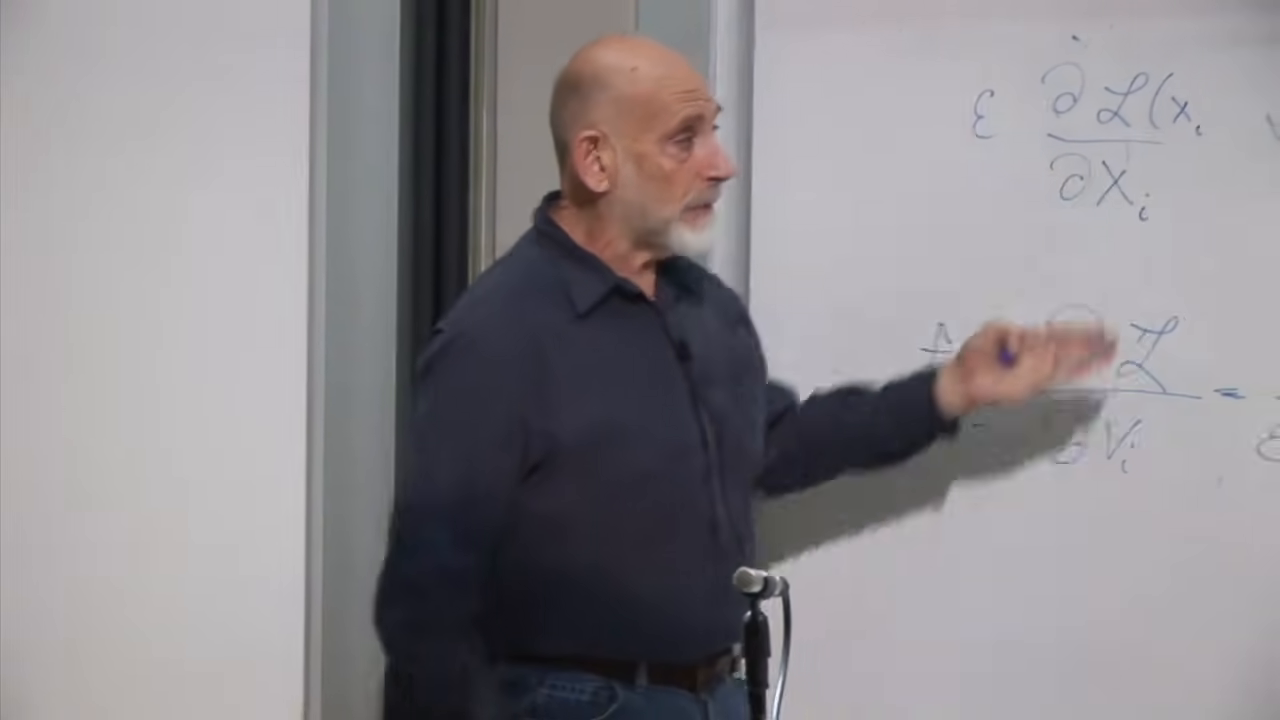
\includegraphics[width=0.74\textwidth]{lecture_03_figure_04.png}
  \caption{La derivada directa respecto de la posición y las dos contribuciones de las derivadas respecto de la velocidad de los intervalos vecinos en la variación discreta.}
  \lectureframe{00:45:26}
\end{figure}

Reordenemos la ecuación ~\eqref{eq:discrete-el-variation}:\begin{equation}
  \frac{1}{\epsilon}
  \left(
    \frac{\partial L_n}{\partial v_n}
    -\frac{\partial L_{n-1}}{\partial v_{n-1}}
  \right)
  =
  \frac{\partial L_n}{\partial x_n}.
  \label{eq:discrete-el}
\end{equation}El lado izquierdo es un cociente de diferencias entre intervalos vecinos. Cuando \(\epsilon\to0\), la línea quebrada se convierte en una trayectoria suave y el cociente se convierte en una derivada temporal:\begin{equation}
  \boxed{
  \frac{d}{dt}\left(\frac{\partial L}{\partial\dot x}\right)
  =
  \frac{\partial L}{\partial x}}
  .
  \label{eq:euler-lagrange-one}
\end{equation}Esta es la ecuación de Euler--Lagrange.

\begin{figure}[htbp]
  \centering
  \includegraphics[width=0.78\textwidth]{lecture_03_figure_11.png}
  \caption{Ecuación de Euler--Lagrange completa, obtenida al imponer la estacionariedad en cada intervalo temporal interior.}
  \lectureframe{00:49:25}
\end{figure}

Una vez especificado \(L\), la ecuación ~\eqref{eq:euler-lagrange-one} funciona como una máquina: se deriva la función dada y se obtiene una ecuación diferencial para la trayectoria.

\begin{classroomqa}\audiencequestion{¿Es válido el resultado de Euler--Lagrange para cualquier función de \(x\) y \(\dot x\)?\lecturetimestamp{00:49:37--00:50:24}}\lecturerresponse{Sí, siempre que se cumpla la regularidad necesaria para las derivadas. El ejemplo de la longitud de arco tiene exactamente la misma forma si se cambia el nombre de su variable independiente \(x\) por el de \(t\), y el de su función incógnita \(y(x)\) por el de \(x(t)\). Su ecuación de Euler--Lagrange tiene soluciones rectilíneas.}\end{classroomqa}

\section{Las ecuaciones de Newton a partir del lagrangiano}

Para una partícula que se mueve en una recta bajo un potencial \(V(x)\), tomemos\begin{equation}
  L(x,\dot x)=T-V
  =\frac12m\dot x^2-V(x).
  \label{eq:lagrangian-tv-one}
\end{equation}El signo menos puede parecer extraño, porque la energía total es \(T+V\). Pero el lagrangiano no es la energía. El criterio es si la máquina de Euler--Lagrange devuelve el movimiento correcto. Se rechaza una votación ficticia sobre el signo: la respuesta hay que comprobarla, no decidirla por votación.

Primero,\begin{equation}
  \frac{\partial L}{\partial\dot x}=m\dot x.
  \label{eq:conjugate-momentum-one}
\end{equation}Esto es el momento lineal. En general, el momento conjugado a cualquier coordenada \(q\) se define como\begin{equation}
  p_q=\frac{\partial L}{\partial\dot q}.
  \label{eq:conjugate-momentum-general}
\end{equation}Al derivar respecto del tiempo la ecuación ~\eqref{eq:conjugate-momentum-one} se obtiene \(m\ddot x\), mientras que\begin{equation}
  \frac{\partial L}{\partial x}
  =-\frac{dV}{dx}.
  \label{eq:lagrangian-position-derivative}
\end{equation}Por tanto, la ecuación de Euler--Lagrange es\begin{equation}
  m\ddot x=-\frac{dV}{dx}=F(x),
  \label{eq:newton-from-action}
\end{equation}que es la segunda ley de Newton.

\begin{figure}[htbp]
  \centering
  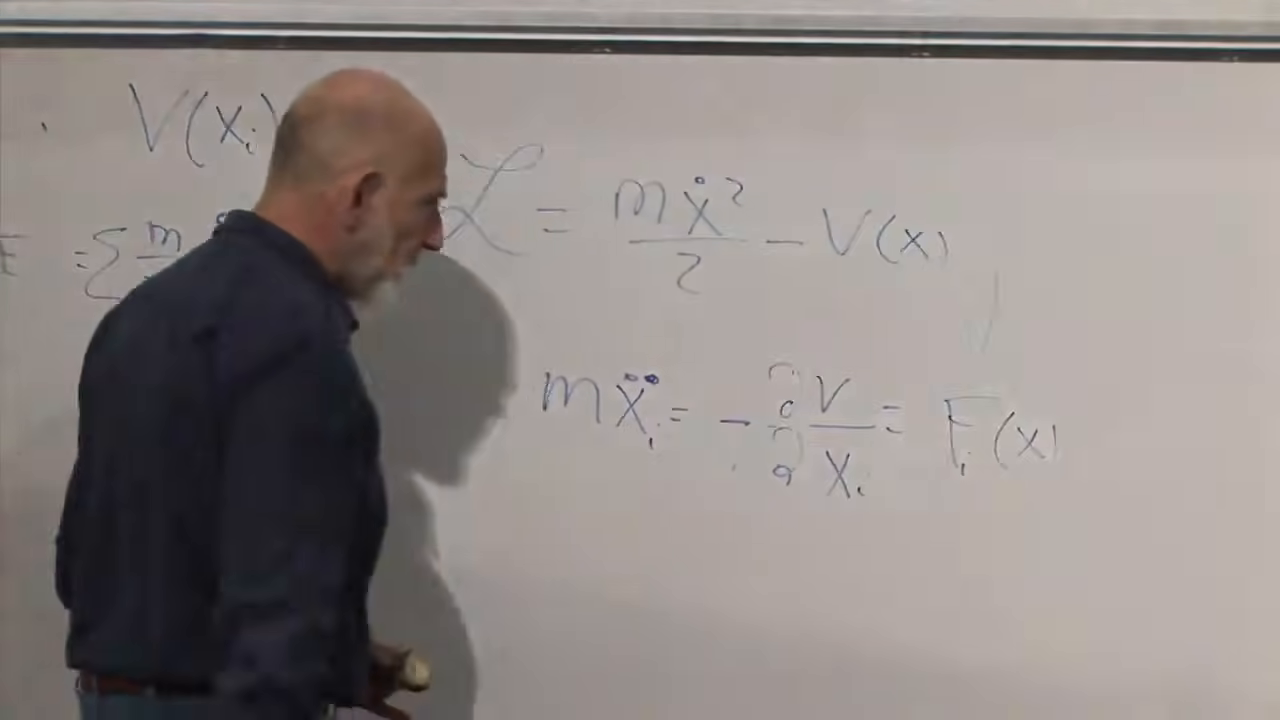
\includegraphics[width=0.80\textwidth]{lecture_03_figure_05.png}
  \caption{Energía cinética, energía potencial, \(L=T-V\) y la forma por componentes recuperada de la ecuación de Newton, todo en una misma pizarra.}
  \lectureframe{00:57:52}
\end{figure}

Para muchas coordenadas \(q_i\),\begin{equation}
  L(\mathbf q,\dot{\mathbf q})
  =\sum_i\frac12m_i\dot q_i^{\,2}-V(q_1,q_2,\ldots),
  \label{eq:lagrangian-tv-many}
\end{equation}y hay una ecuación para cada coordenada:\begin{equation}
  \frac{d}{dt}\left(\frac{\partial L}{\partial\dot q_i}\right)
  =\frac{\partial L}{\partial q_i}
  \quad\Longrightarrow\quad
  m_i\ddot q_i=-\frac{\partial V}{\partial q_i}=F_i.
  \label{eq:euler-lagrange-many}
\end{equation}La trayectoria sigue siendo una sola curva, ahora en un espacio de configuración de muchas dimensiones.

\begin{classroomqa}\audiencequestion{¿Hemos trabajado simplemente hacia atrás desde la ley de Newton y diseñado un funcional que reproduce la respuesta?\lecturetimestamp{00:58:07--01:00:04}}\lecturerresponse{Esa no es la perspectiva más fructífera. El lagrangiano es la especificación compacta del sistema físico: una función de todas las coordenadas y velocidades reúne todas sus ecuaciones de movimiento. En las teorías nuevas, los físicos suelen proponer una acción y deducir las ecuaciones, en vez de adivinar cada ecuación por separado.}\end{classroomqa}

Esta forma compacta de reunir las ecuaciones es una ventaja. La libertad de coordenadas es otra. La afirmación de que una línea es la más corta no depende de que el plano se describa con coordenadas cartesianas, polares o curvilíneas. Del mismo modo, la estacionariedad de la acción es independiente de las coordenadas, aunque cambien la expresión de \(L\) y las ecuaciones resultantes por componentes.

\section{Una partícula libre vista desde un carrusel}

Sean \((x,y)\) las coordenadas cartesianas inerciales y \((X,Y)\) las coordenadas cartesianas que giran uniformemente con velocidad angular \(\omega\). Con la orientación usada aquí,\begin{align}
  x&=X\cos\omega t+Y\sin\omega t,
  \notag\\
  y&=-X\sin\omega t+Y\cos\omega t.
  \label{eq:rotating-coordinate-map}
\end{align}El ángulo entre los sistemas de referencia es \(\omega t\).

\begin{figure}[htbp]
  \centering
  \includegraphics[width=0.76\textwidth]{lecture_03_figure_12.png}
  \caption{Ejes cartesianos inerciales y giratorios uniformemente. Un mismo punto recibe coordenadas giratorias que dependen del tiempo.}
  \lectureframe{01:06:05}
\end{figure}

Una partícula libre tiene el lagrangiano, en el sistema inercial,\begin{equation}
  L_{\mathrm{in}}
  =\frac{m}{2}\left(\dot x^2+\dot y^2\right).
  \label{eq:free-inertial-lagrangian}
\end{equation}Derivemos la ecuación ~\eqref{eq:rotating-coordinate-map} y usemos \(\sin^2\omega t+\cos^2\omega t=1\). Los términos trigonométricos se combinan y dan\begin{align}
  \dot x^2+\dot y^2
  &=
  \dot X^2+\dot Y^2\\
  &\quad+\omega^2(X^2+Y^2)\\
  &\quad+2\omega(Y\dot X-X\dot Y).
  \label{eq:rotating-speed}
\end{align}Así,\begin{align}
  L_{\mathrm{rot}}
  &=
  \frac{m}{2}(\dot X^2+\dot Y^2)\\
  &\quad+\frac{m\omega^2}{2}(X^2+Y^2)\\
  &\quad+m\omega(Y\dot X-X\dot Y).
  \label{eq:rotating-lagrangian}
\end{align}

\begin{figure}[htbp]
  \centering
  \includegraphics[width=0.84\textwidth]{lecture_03_figure_13.png}
  \caption{El lagrangiano transformado de la partícula libre: energía cinética ordinaria, un término centrífugo cuadrático y un término lineal en la velocidad.}
  \lectureframe{01:12:16}
\end{figure}

El término cuadrático en las coordenadas tiene la forma \(-V_{\mathrm{fict}}\), donde\begin{equation}
  V_{\mathrm{fict}}
  =-\frac{m\omega^2}{2}(X^2+Y^2).
  \label{eq:centrifugal-potential}
\end{equation}Disminuye hacia afuera, por lo que produce la fuerza centrífuga \(m\omega^2(X,Y)\).

El último término de la ecuación ~\eqref{eq:rotating-lagrangian} es lineal tanto en las coordenadas como en las velocidades. Al aplicar la ecuación de Euler--Lagrange se obtiene\begin{align}
  m\ddot X&=m\omega^2X-2m\omega\dot Y,
  \notag\\
  m\ddot Y&=m\omega^2Y+2m\omega\dot X.
  \label{eq:rotating-equations}
\end{align}Los términos proporcionales a \(\omega^2\) son centrífugos; los proporcionales a la velocidad son de Coriolis. En forma vectorial, dentro del plano giratorio,\begin{equation}
  \mathbf F_{\mathrm{C}}
  =-2m\,\boldsymbol\omega\times\mathbf v_{\mathrm{rot}},
  \label{eq:coriolis-vector}
\end{equation}con los signos ajustados si se elige la convención de orientación opuesta.

\begin{figure}[htbp]
  \centering
  \includegraphics[width=0.84\textwidth]{lecture_03_figure_14.png}
  \caption{Ecuaciones en el sistema giratorio: los términos proporcionales a las coordenadas producen aceleración centrífuga, mientras que los términos cruzados de velocidad producen aceleración de Coriolis.}
  \lectureframe{01:20:20}
\end{figure}

La cuestión no es que el álgebra desaparezca. Es que una sola transformación de coordenadas aplicada a una única función escalar genera las dos ecuaciones acopladas y las dos fuerzas ficticias.

\begin{classroomqa}\audiencequestion{¿Funciona este método con coordenadas de curvatura arbitraria?\lecturetimestamp{01:22:01--01:22:17}}\lecturerresponse{Sí. Las nuevas coordenadas pueden ser curvilíneas e incluso depender explícitamente del tiempo, como ocurre con las coordenadas giratorias. Reescribimos la acción en las nuevas variables y aplicamos la misma regla de Euler--Lagrange.}\end{classroomqa}

\section{Coordenadas polares y un ángulo cíclico}

Para las coordenadas polares ordinarias,\begin{equation}
  x=r\cos\theta,
  \qquad
  y=r\sin\theta.
  \label{eq:polar-map}
\end{equation}Tanto \(r\) como \(\theta\) pueden variar con el tiempo. Al derivar y sumar los cuadrados se obtiene\begin{equation}
  \dot x^2+\dot y^2
  =\dot r^2+r^2\dot\theta^2.
  \label{eq:polar-speed}
\end{equation}Para un potencial central \(V(r)\),\begin{equation}
  L
  =\frac{m}{2}\left(\dot r^2+r^2\dot\theta^2\right)-V(r).
  \label{eq:polar-lagrangian}
\end{equation}

\begin{figure}[htbp]
  \centering
  \includegraphics[width=0.80\textwidth]{lecture_03_figure_15.png}
  \caption{Geometría polar y descomposición de la energía cinética en movimiento radial y angular.}
  \lectureframe{01:23:30}
\end{figure}

La ecuación radial es\begin{equation}
  m\ddot r
  =mr\dot\theta^2-\frac{dV}{dr}.
  \label{eq:radial-equation}
\end{equation}El primer término es la contribución centrífuga hacia afuera asociada al movimiento angular de la propia partícula.

Para el ángulo,\begin{equation}
  \frac{d}{dt}\left(\frac{\partial L}{\partial\dot\theta}\right)
  =\frac{\partial L}{\partial\theta}=0,
  \label{eq:theta-el}
\end{equation}porque el potencial central no depende explícitamente de \(\theta\). Por tanto,\begin{equation}
  \frac{d}{dt}\left(mr^2\dot\theta\right)=0,
  \qquad
  mr^2\dot\theta=\ell,
  \label{eq:angular-momentum}
\end{equation}donde \(\ell\) es el momento angular conservado.

\begin{figure}[htbp]
  \centering
  \includegraphics[width=0.82\textwidth]{lecture_03_figure_16.png}
  \caption{La ecuación angular de Euler--Lagrange tiene el lado derecho nulo, lo que revela la conservación de \(mr^2\dot\theta\).}
  \lectureframe{01:29:25}
\end{figure}

La ecuación angular da\begin{equation}
  \dot\theta=\frac{\ell}{mr^2}.
  \label{eq:theta-dot-angular-momentum}
\end{equation}Al sustituir en la ecuación ~\eqref{eq:radial-equation} queda una sola ecuación para \(r\):\begin{equation}
  m\ddot r
  =\frac{\ell^2}{mr^3}-\frac{dV}{dr}.
  \label{eq:effective-radial-equation}
\end{equation}

Tradicionalmente, se llama \emph{cíclica} a una coordenada que no aparece en \(L\), aunque no sea un ángulo. Si \(q\) es cíclica, entonces\begin{equation}
  \frac{\partial L}{\partial q}=0
  \quad\Longrightarrow\quad
  \frac{d}{dt}\left(\frac{\partial L}{\partial\dot q}\right)=0.
  \label{eq:cyclic-conservation}
\end{equation}Su momento conjugado se conserva. Esta es la primera muestra de un vínculo general entre simetría y ley de conservación.

\section{Preguntas sobre el significado, la energía y el alcance}

Las preguntas que siguen ponen de manifiesto dónde reside el contenido más profundo del formalismo.

\begin{classroomqa}\audiencequestion{¿Hay una razón independiente para llegar al lagrangiano, más allá de descubrir que da las ecuaciones clásicas correctas?\lecturetimestamp{01:33:25--01:35:07}}\lecturerresponse{Históricamente, más de un siglo de mecánica clásica mostró que las partículas, las ondas y los campos electromagnéticos podían expresarse todos de esta forma. En el ámbito clásico, ese éxito acumulado es un hecho empírico acerca de cómo se organizan las leyes. La explicación más profunda proviene de la mecánica cuántica y se deja para más adelante.}\end{classroomqa}

\begin{classroomqa}\audiencequestion{En el lagrangiano del sistema giratorio, ¿se puede asignar al término lineal en la velocidad una energía cinética o potencial ordinaria?\lecturetimestamp{01:35:08--01:36:23}}\lecturerresponse{No. La cantidad conservada asociada a las traslaciones temporales se obtiene mediante la construcción del hamiltoniano, no interpretando cada término de \(L\) como energía cinética o potencial. Para la ecuación ~\eqref{eq:rotating-lagrangian}, el término lineal en la velocidad se cancela en \(\sum_a\dot q_a\,\partial L/\partial\dot q_a-L\). El tratamiento hamiltoniano organizará esto de manera sistemática.}\end{classroomqa}

En efecto, como \(L_{\mathrm{rot}}\) no depende explícitamente del tiempo,\begin{equation}
  \begin{aligned}
    H_{\mathrm{rot}}
    &=\dot X\frac{\partial L}{\partial\dot X}
     +\dot Y\frac{\partial L}{\partial\dot Y}-L\\
    &=\frac{m}{2}(\dot X^2+\dot Y^2)
     -\frac{m\omega^2}{2}(X^2+Y^2)
  \end{aligned}
  \label{eq:rotating-hamiltonian-preview}
\end{equation}se conserva. Es la integral de Jacobi en el sistema giratorio, y no la misma energía numérica que asigna el observador inercial. Los cambios de coordenadas dependientes del tiempo no tienen por qué conservar la forma numérica de la energía.

\begin{classroomqa}\audiencequestion{¿Y si la trayectoria curva se debe a la gravedad?\lecturetimestamp{01:36:30--01:37:10}}\lecturerresponse{Para la gravedad newtoniana, basta con usar \(V(r)=-GMm/r\) en el lagrangiano de fuerza central. El espacio-tiempo curvo pertenece a la relatividad general y aquí no se presupone.}\end{classroomqa}

\begin{classroomqa}\audiencequestion{¿Son meramente ficticios el potencial centrífugo y su energía?\lecturetimestamp{01:37:13--01:40:14}}\lecturerresponse{Un observador sobre la plataforma giratoria mide las fuerzas efectivas y puede usar de forma coherente la cantidad conservada del sistema giratorio. «\emph{Ficticio}» significa que estos términos surgen de una descripción no inercial, no que sus efectos observados sean imaginarios. La energía misma no es invariante ante un cambio general de coordenadas dependiente del tiempo.}\end{classroomqa}

\begin{classroomqa}\audiencequestion{¿En qué dirección apunta la fuerza de Coriolis, que depende de la velocidad?\lecturetimestamp{01:40:22--01:42:36}}\lecturerresponse{Es perpendicular a la velocidad en el sistema giratorio, y su magnitud es proporcional a la rapidez y a la velocidad angular del sistema de referencia. En el plano, las componentes intercambian \(\dot X\) y \(\dot Y\) con signos opuestos, como en la ecuación ~\eqref{eq:rotating-equations}.}\end{classroomqa}

\begin{figure}[htbp]
  \centering
  \includegraphics[width=0.76\textwidth]{lecture_03_figure_17.png}
  \caption{Patrón de las componentes cruzadas de la velocidad: la fuerza de Coriolis es perpendicular a la velocidad en el sistema giratorio.}
  \lectureframe{01:41:40}
\end{figure}

\begin{classroomqa}\audiencequestion{¿Es necesario expresar el lagrangiano inicial en un sistema inercial?\lecturetimestamp{01:42:37--01:44:00}}\lecturerresponse{Para una partícula libre ordinaria, la ley de Newton en un sistema inercial proporciona la forma inicial sencilla \(m(\dot x^2+\dot y^2)/2\). Una vez conocida esa ley física, se puede transformar la acción a cualquier otro sistema de coordenadas. No se debe suponer, de manera independiente, la misma fórmula cinética sencilla en un sistema giratorio.}\end{classroomqa}

El mismo tipo de término lineal en la velocidad aparece para una partícula cargada en un campo magnético:\begin{equation}
  L_{\mathrm{em}}
  =\frac12m\mathbf v^2
   +q\mathbf A(\mathbf r,t)\cdot\mathbf v
   -q\phi(\mathbf r,t).
  \label{eq:electromagnetic-lagrangian}
\end{equation}Para un campo magnético uniforme perpendicular al plano, el gauge simétrico \(\mathbf A=\tfrac12\mathbf B\times\mathbf r\) produce un término proporcional a \(X\dot Y-Y\dot X\), con la misma estructura algebraica que el término de Coriolis.

\begin{figure}[htbp]
  \centering
  \includegraphics[width=0.82\textwidth]{lecture_03_figure_18.png}
  \caption{El término lineal en la velocidad del sistema giratorio que motiva la comparación con una partícula cargada en un campo magnético uniforme.}
  \lectureframe{01:44:40}
\end{figure}

\begin{classroomqa}\audiencequestion{¿Hay restricciones, aparte de la suavidad, sobre qué función puede servir de lagrangiano?\lecturetimestamp{01:44:46--01:45:06}}\lecturerresponse{Sí, pero las restricciones pertinentes requieren una estructura que aún no hemos desarrollado, así que se dejan para más adelante. En esta etapa, la lección central es cómo un lagrangiano propuesto genera ecuaciones y leyes de conservación.}\end{classroomqa}

Las ecuaciones del sistema giratorio también admiten movimiento circular: desde el carrusel, se ve que un punto fijo en el sistema inercial gira alrededor del origen rotatorio. La analogía magnética explica entonces por qué una partícula cargada puede realizar un movimiento ciclotrónico circular.

\begin{classroomqa}\audiencequestion{¿La partícula cargada permanecería en esa órbita circular o la radiación haría que colapsara?\lecturetimestamp{01:46:11--01:47:21}}\lecturerresponse{Las ecuaciones que consideran solo la partícula y que estamos analizando omiten la radiación. Al incluir el acoplamiento al campo electromagnético y la reacción de radiación, una carga clásica acelerada puede radiar. Por tanto, la radiación es un efecto físico adicional, no una contradicción de la órbita en las ecuaciones truncadas.}\end{classroomqa}

\begin{classroomqa}\audiencequestion{¿Qué papel tienen los huracanes en esta discusión?\lecturetimestamp{01:47:30--01:47:50}}\lecturerresponse{El movimiento atmosférico a gran escala tiene lugar sobre la Tierra en rotación, así que los efectos de Coriolis son importantes. Una derivación adecuada pertenece a la meteorología y no se intenta aquí.}\end{classroomqa}

\begin{classroomqa}\audiencequestion{¿Se espera que el marco de la acción abarque todas las leyes físicas, y qué supondría una excepción genuina?\lecturetimestamp{01:47:57--01:49:01}}\lecturerresponse{Todas las teorías fundamentales cerradas conocidas dentro del alcance de esta discusión pueden organizarse mediante una acción: las partículas newtonianas, los campos de Maxwell, la relatividad general y el modelo estándar. Los aparentes contraejemplos, como el rozamiento viscoso, surgen cuando se omiten grados de libertad del entorno. Si se amplía el sistema para incluir el fluido o el baño microscópico, la descripción fundamental vuelve a encajar en este marco. Por tanto, una excepción verdaderamente fundamental sería un gran descubrimiento.}\end{classroomqa}